\subsubsection{Design of Registers} \label{sec:design-registers}

As mentioned in Section \ref{sec:design-instruction-set}, in ZKVM, we not only have to constrain the state of the registers associated with
the instruction to be updated correctly, but we also have to constrain the state of the registers not involved in the current
instruction to remain unchanged.Even though register-based VMs have certain advantages, from the verification point of view,
it is not better to have a larger number of registers; there is a trade-off to be considered:

\begin{itemize}
    \item How many registers will be sufficient for most of the calculations?
    \item For some calculations, is the increased number of memory accesses acceptable when there are not enough registers?
\end{itemize}

If the number of registers is small enough and at the same time the memory accesses introduced do not yet need to be constrained,
this would be the ideal case from the point of view of verification efficiency, as in the design of the \href{https://starkware.co/cairo/}{Cairo VM}, where there are
no general-purpose registers and all operands of the instruction originate from memory;at the same time, to avoid consistency checks
on memory, the write-once model is used, since memory cannot be rewritten at the execution level, so checks are not needed.

However, the downside of introducing the write-once model is that it is not friendly to Dapps developers, and the limitations of
the memory model make it necessary for developers to pay special attention to the way memory is used when developing Dapps.
(the traditional memory model is the read-write model).

\begin{figure}[!ht]
    \centering
    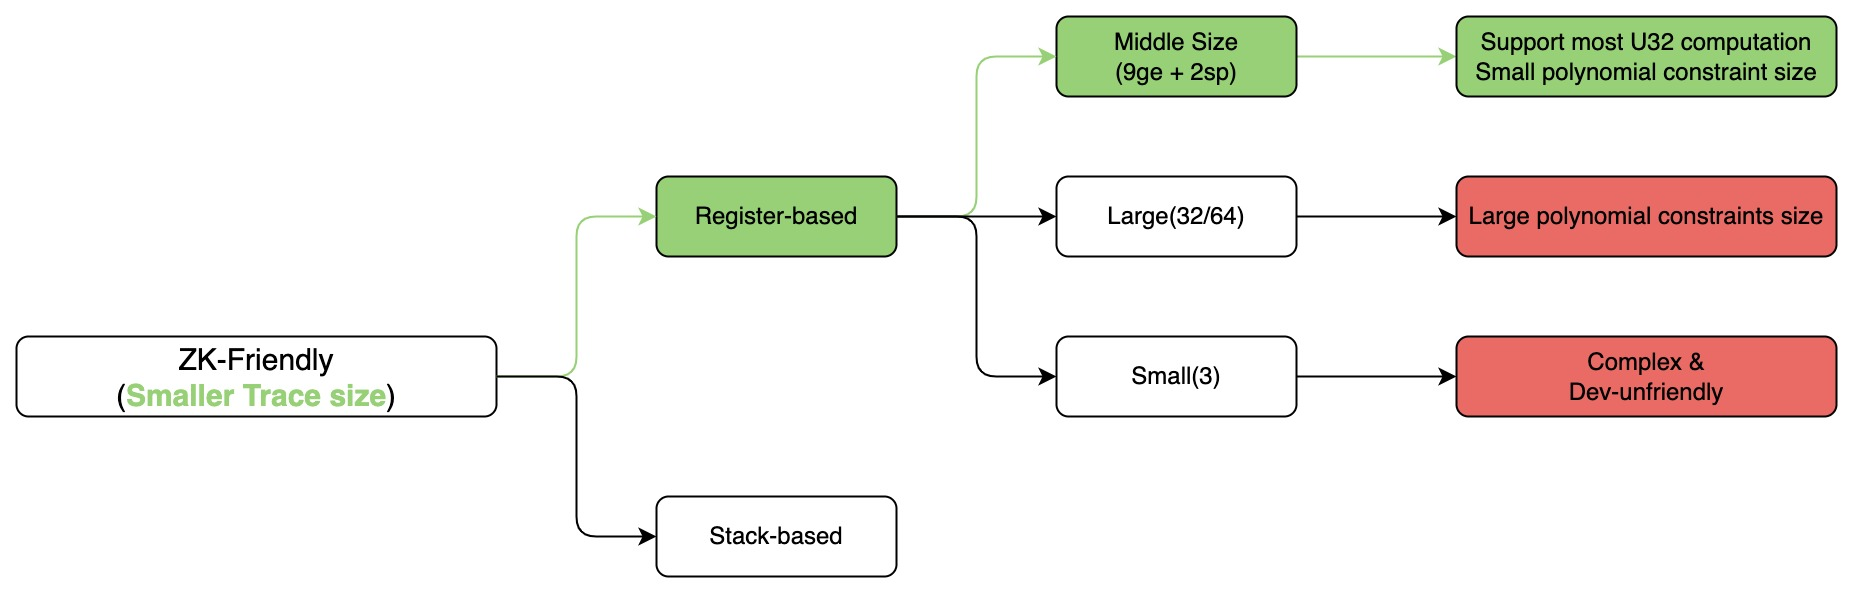
\includegraphics[width=0.6\textwidth]{vm/design-zk-friendly-register.jpeg}
    \caption{How to get ZK-Friendly(Smaller Trace) from register}
    \label{fig:design-zk-friendly-register}
\end{figure}

As shown in \figref{fig:design-zk-friendly-register}, we choose an optimal solution from both ZK-Friendly and Dev-Friendly perspectives.In terms of the number of
registers, considering that the minimum type of computation supported on OlaVM is U32 integer computation, plus some boundary conditions,
such as the number of loops, loop termination conditions, etc, nine general-purpose registers can support most of the U32 computation
(both U64 and U256 integer computation can be implemented through the U32 library), and 2 special registers (PC, PSP) is used in OlaVM, reference: Section \ref{subsec: instructions-set}.
When the number of registers is not enough, memory is needed for caching, so memory access-related instructions
(MLOAD, MSTORE) will be added, but it is worth noting that in order to facilitate the FFT, Prover often adds redundant data in Trace to meet
the size of Trace to the power of 2. be replaced with valid data, as shown in \figref{fig:design-better-trace-layout}.

\begin{figure}[!ht]
    \centering
    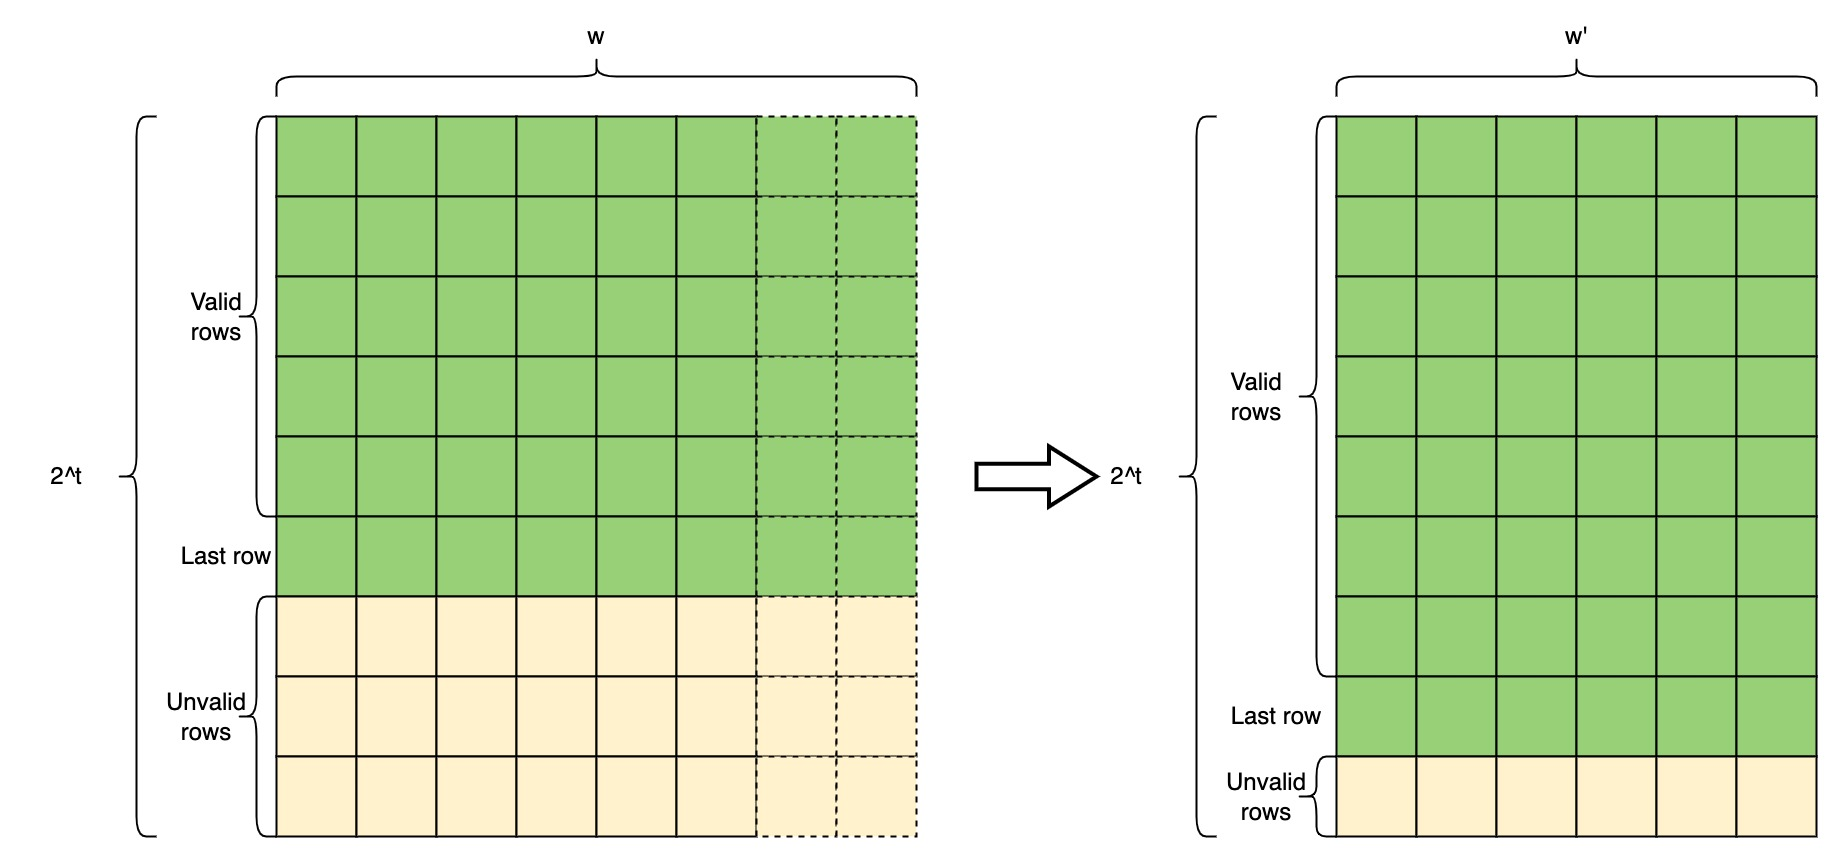
\includegraphics[width=0.6\textwidth]{vm/design-better-trace-layout.jpeg}
    \caption{Better layout of Trace}
    \label{fig:design-better-trace-layout}
\end{figure}
